%---------------------------------------------------------------------------------------
\section{Abstract}	% Section headings need to be upper and lower case.
%---------------------------------------------------------------------------------------
\addtocounter{section}{1}


% Globally distributed internet services are ubiquitous today. These services are driving the demand to build mega-watt scale data center facilities (DC) distributed through out the globe. 

Over the last decade, operational efficiency optimizations in data center (DC) facilities designs have curtailed their absolute power demands. However, in absolute terms their physical footprint is still growing. Offsetting effects such as the these make system level life cycle environmental footprint evaluations complex for distributed services operating in these DCs. 

To support system level evaluations for service operating in DCs, this research uses simulated network traffic and coincident energy generation source aware building energy models (BEM) to evaluate the marginal carbon footprint of a globally spanning network of data centers. The result of this research is a BEM based framework that can be used in environmental decisions to characterize their life-cycle costs.




%---------------------------------------------------------------------------------------
\section{Introduction}
%---------------------------------------------------------------------------------------
Globally distributed internet services are ubiquitous today. These services are driving the demand to build mega-watt scale data center facilities (DC) distributed through out the globe. In a 2015 study data centers were forecast to consume as much as 13\% of the global energy production by 2030 \citep{andrae15}. More optimistic models form the US Department of Energy for the US showed a curtailment with up to fifty percent decline in energy compared to the industry's use of 2\% of the power produced by the national grid in 2005 as a result of using state of the art efficiency and consolidation practices \citep{Shehabi16}. As more and more parts of society are transitioning to data center dependent online paradigms, the absolute demand of data centers is growing. The volume of growth is exemplified by the capital costs being invested across the world in constructing these data centers.

The growth in data center capital construction costs will reach \$89 billion by 2027, a significant increase from the \$45 billion spent in 2018 \citep{dcmarket19}. Capital costs aren’t the only commitments for data center owners however. DC owner\textsc{\char13}s also incur significant operational costs throughout the entire operational lives of their facilities.  

Over a 20-year life of a continuously operating data-center facility, the use-phase energy costs can exceed its capital costs while having a much larger ecological footprint. Given the accumulation of costs and impacts over the life of data centers, there is a need for a robust model the couples the information technology (IT) and building systems with their energy supply sources through its useful life. In this article a geographically extensible model that accounts for the workloads, building systems, and power utility grid is presented.

In the rest of this paper a model for coincident energy demand and marginal energy costs (MEC) of a set of data centers is proposed and developed. First, the proposed method uses a hybrid model consisting of EnergyPlus and Python programming modules as developed by the researcher in \citep{kumar20}. For this article, the researcher's original hybrid model is modified as described in the methodology section to be more indicative of the current operations of cloud data centers. Then second, the resulting time series of operational energy demand profile is used as input to a Python based open source MEC simulation tool that is also extended as described in the methodology section. The baseline MEC model is described next. 

The MEC calculations are based on the Dispatch Optimized Systems Cost of Energy (DOSCOE) model developed by Platt \citep{platt17}. DOSCOE provides a linear programming platform that computes the monetary costs and several environmental emissions associated with operating a mix of dispatch-able and non-dispatch-able energy sources. In this context, dispatch-able energy sources are those that can be controlled to meet demand. Natural gas power plants are examples of dispatch-able source of energy, where the plant operators can control the mass flow rates of the combustion gases to curtail generation rates. On the contrary are the non-dispatchable sources, where the energy generation is dependent on extrinsic factors. An example of non-dispatchable energy source is solar; where cloud cover greatly effects the generation rate and no power can be generated at night.

Modeling the costs for a mixture of dispatchable and non-dispatchable generators is complex as most non-dispatchable sources are only accounted for as opportunistic supply sources when sizing the power generation infrastructure. By dsign the dispatchable generators are sized to meet the full demand in a worst-case condition when no dispatchable power is available \citep{platt17}. However, when non-dispatchable power is opportunistically available, it supplements the grid; allowing dispatchable sources to be turned down to part loads. This saves fuel costs for dispatchable sources (ie natural gas generators), but it leaves their physical infrastructure stranded and underutilized. This research’s coupling of the DOSCOE model with a BEM quantifies the monetary and ecological costs associated with operating data centers in grids with optimal mixtures of energy sources bound by physical constraints to be evaluated by matching the marginal costs of energy with data center demands on hourly intervals. Furthermore, the resulting model is inclusive of the stranded costs of the underutilized power infrastructure.

In the next section, Background, informative context is provided to set the proper use-case for this framework. Then in the Similar Works section, past literature which have quantified the ecological life cycle cost of data centers and internet services are summarized. In the Methodology section, the two main modules of the software implementation of this research are presented. Specifically these modules are a modified version of hybrid building energy model and a novel MEC model based on DOSCOE. After the details of the models are presented, the results are discussed in the Results and Discussion section followed by the Conclusions.


%---------------------------------------------------------------------------------------
\section{Background}
%---------------------------------------------------------------------------------------
Data centers are critical to modern internet experiences for billions of people. They are the key enablers for disseminating information in real time regardless of people's location. As an example of location agnostic services geographical dispersed infrastructure, Figure~\ref{fig:net_diag} illustrates a geographically distributed architecture that enables data centers to provide globally consistent internet experience that have become the status quo over the last decade. Distributed software architectures implemented in the server clusters at the leaf-nodes consist of a collection of autonomous computing resources that appear to its users as a single coherent system \citep{tanenbaum}.

In Figure~\ref{fig:net_diag}, a data center network stack with three hierarchical WAN layers are shown. The first hierarchical layer, the global level, has a wide area network (WAN) connected to two internet service providers (ISP) as its root node. For the purposes of this work the WAN is an abstraction of a network that connects a set of data center facilities with each other. The second layer of the global level are the metropolitan regions. In this layer, the ISP links are shown as coming in from top and the outgoing links from the bottom serve local distribution networks to buildings within the metropolitan areas. The final layer of the global level are the data center buildings, where the global network links connect to clusters of servers. Inside each data center there may be another independent hierarchy as shown by the server clusters. The physical network links shown in Figure~\ref{fig:net_diag} connect the buildings to each other through the WAN. However, the physical links (Pink, Magenta) is transparent for the clusters, which directly communicate with each other through logical links (Gray, Green, Red).

\begin{figure}
  \centering
  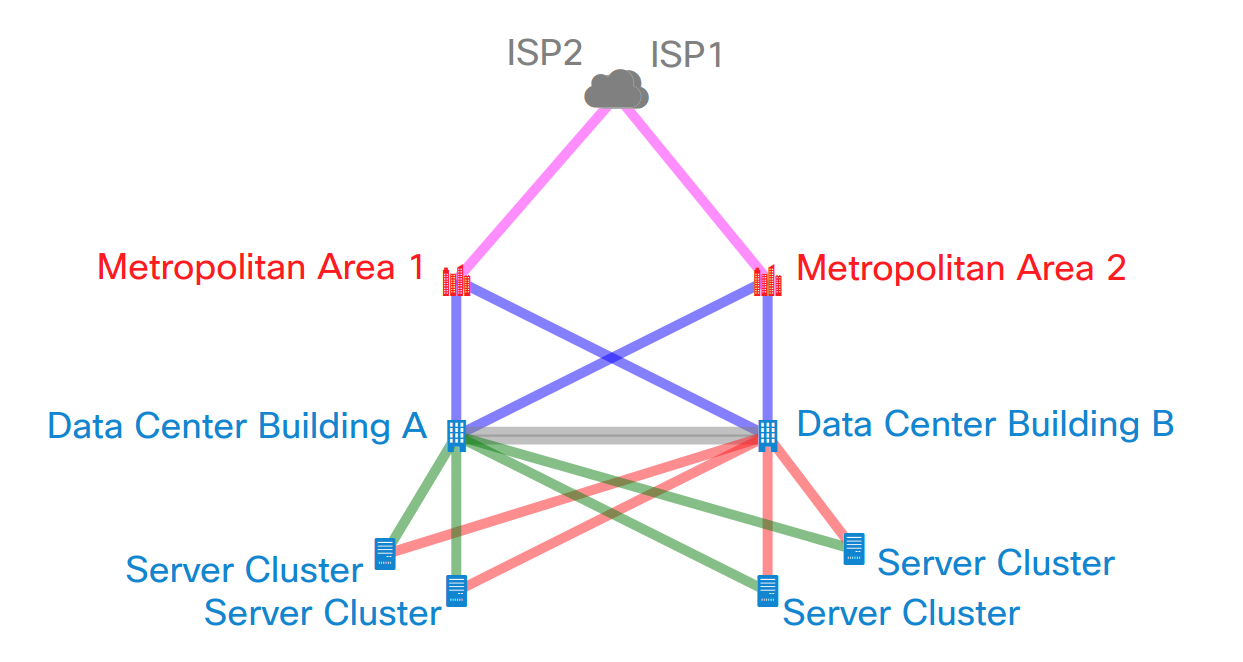
\includegraphics[scale=.2]{marginal_energy_cost/img/net_diag.png}
  \caption[Generic Network Topology]{General Topology of data center networks. The 1:1 metropolitan area to building relationships are shown for clarity only. Pink: indicates the first layer - ISP-Metropolitan links (physical). Magenta: indicates the second layer Metropolitan-DC Building with a full mesh connection (physical). Gray: represents the cross-connection between Data Centers (logical). Green/Red: Cluster to Cluster links (logical).}
  \label{fig:net_diag}
  \end{figure}


Large cloud data center operators have championed WAN systems for global up-time (service availability) and user experience optimizations \citep{sushant13} \citep{hong13}. Cloud data centers are a specific class of data centers. They serve business functions that require custom IT and building systems tuned for optimality in total costs of ownership models. These facilities house numerous services that can be controlled by network load balancers, with each data center limited by its physical infrastructure's capacity. As described in Sushant and Hong, the WAN networks can shift loads between data center on command.  The efficacy of a strategy for shifting computational loads depends on the capacity headroom of the physical resources at the data center where the loads are shifted to. 

The fungibility of locations enabled by WANs is desirable from an service application performance point of view as latency can be significantly reduced for specific markets and applications by minimizing the round trip communication times with consumers. Given the popularity of the public clouds, the use of network aware energy models for data centers extends beyond just data center construction and plant operations. Extending beyond the physical data center, network aware energy models can be used by internet services that operate public clouds where a given service is sharing the resources with may other independent services.    

In the context of BEMs, WAN's make the IT workloads temporally (and geographically) unstable, rendering it elusively for building modelers to reason about. As an example of temporal and geographical instability of data centers, Figure~\ref{fig:google_activity_dist} \citep{barroso18} shows the difference in utilization rates for two server clusters from Barroso's operational experience. This behavior of IT loads is something that WAN aware BEMs can help characterize and exploit. One possible means of exploitation is to flatten the peak of each cluster by routing the excessive workloads to another similarly provisioned cluster with lower coincident demands and sufficient building systems capacity headroom. However, building energy simulation need to be aware of more then just energy to make the right environmental decisions. To effectively optimize environmental objectives, BEMs coupled with MEC models can quantify the energy's global warming potential in terms of carbon footprint to shift loads from one building to another.

  \begin{figure}
    \centering
    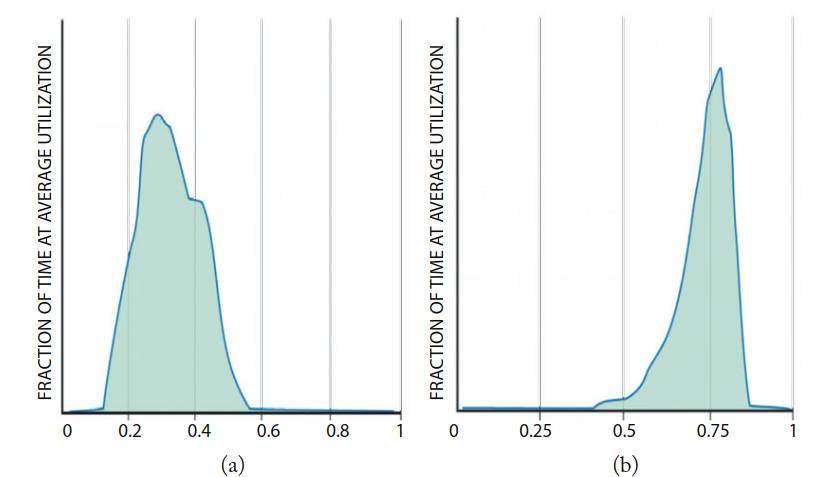
\includegraphics[scale=.2]{marginal_energy_cost/img/google_activity_dist.png}
    \caption[Usage profiles of two production DC Clusters]{Activity distribution of a sample of 2 clusters, each containing over 20,000 servers, over a period of 3 months. The x-axis indicates the server utilization rates (0 to 1) and the y-axis indicates the fraction of time during the 3 months \citep{barroso18}. The figure on the right (b) shows that peak utilization exceeds 75\% with little variances over the 3 months, whereas the right figure (a) shows that utilization is below 60\% at all times.}
    \label{fig:google_activity_dist}
    \end{figure}

Based on the literature reviews and references cited, there are no publicly available simulation frameworks that couple the dynamic data center workloads and the coincident carbon footprint associated with powering their load. The marginal cost of energy coupled building energy model described in this research is the first publicly available tool to allow owners, designers, and researchers to quantify the carbon footprint of data center operations accounting for granular supply and demand matching of power. Next, a literature review of past works concerning the carbon footprint of data-centers and digital services is presented in the Similar Works section.


%---------------------------------------------------------------------------------------
\section{Similar Works}
%---------------------------------------------------------------------------------------
There are two notable past works that look at the energy footprint for distributed sets of data centers. First, Tripadi considers hardware capital costs alongside with energy acquisition costs to quantify the total costs of ownership in \citep{tripadi17}. Tripadi\textsc{\char13}s framework is dynamic in terms of workloads but it is not aware of the building energy dynamics. In the second work, Kiani and Ansari describe a geographical load balancing strategy that exploits green energy mix in the utility grid \citep{kiani17}. However, their load balancing scheme doesn\textsc{\char13}t provide insights into how the load balancer evaluates the building energy demands or how the greenness of the energy supply is obtained. 

Using a life cycle assessment framework, Whitehead demonstrates a comprehensive data center site level life cycle costs analysis in \citep{whitehead15}. All energy use in Whitehead’s models were deduced from annualized PUE values, precluding coincident energy source evaluations with their framework. Similarly the Green Grid’s data center life cycle assessment guideline is limited to PUE as their suggested basis for the operational energy proxy \citep{tgg12}. The PUE metric is shown in Equation~\ref{eq:pue}, it has proven to be the most popular method for data center operational efficiencies since 2006 \citep{wiki_pue}.

    \begin{equation} \label{eq:pue}
    PUE=\frac{E_{total}}{E_{IT}} 
    \end{equation}
    \begin{center}
    $E_{total}$ = Total Power Used at Facility
    
    $E_{IT}$ = Power Consumed by IT Equipment
    \end{center}
    \vspace{.2cm}
    

Other’s have evaluated the costs of internet services \citep{koomey08} \citep{shehabi14}. Taylor and Koomey quantify the energy and greenhouse gas implications of online Advertising circa 2008. While Shehabi evaluates the energy and greenhouse gas implications of video stream circa 2014 \citep{shehabi14}. Together these works provide a taxonomy that can be followed to assess internet service costs in terms of energy use. 

%---------------------------------------------------------------------------------------
\section{Methodology}
%---------------------------------------------------------------------------------------
In this section the MEC model\textsc{\char13}s coupling with the BEM is described. The resulting model maintains a strict partition between the two technical domains. The first part of the model simulates the hourly energy demands of a set of five data centers in EnergyPlus (EP) using the method demonstrated in \citep{kumar20}. These data centers are distributed across the globe as shown in Figure~\ref{fig:dc_locations}. Then in the second part, the data center demands are matched with the respective region\textsc{\char13}s utility power generation sources for the coincident hour to assess the MEC during that hour. These parts are described in the following subsections. 

\begin{figure}
  \centering
  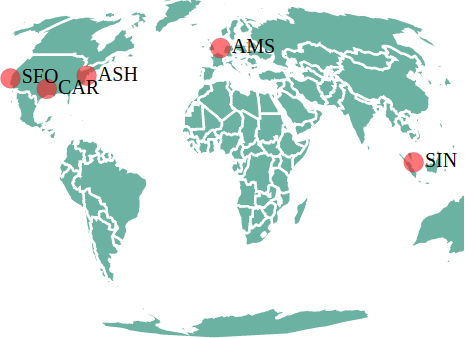
\includegraphics[scale=.40]{marginal_energy_cost/img/dc_locations.png}
  \caption{Data center locations}
  \label{fig:dc_locations}
  \end{figure}

A fundamental component of the demonstrated implementation of this framework is the network traffic simulator from \citep{kumar20}. The simulation produces a time-series profile of the network traffic that a hypothetical service will get at a particular data center site. The hypothetical services are based on Wikipedia and segregated according to the natural language of the Wikipedia pages. By segregating services by natural languages allows the treatment of each language as a 'service platform'. With these network simulations, one or more languages can be supported from a single data center with the constraint that the sum of the IT workloads does not exceed the capacity of the data center facility. 

%---------------------------------------------------------------------------------------
\subsection{Building Energy Model}
%---------------------------------------------------------------------------------------
For the first part, a sufficient building energy demand profile is simulated as in \citep{kumar20}.  The IT workload profile characterizing the power and cooling load is obtained by using simulating the 50th quantile of daily network traffic to each data center using Kumar’s method from \citep{kumar20b}.  However in lieu of using EP release 8.6, the simulation in this work uses EP release 8.9. The changes found EP 8.9 are listed in NREL’s GitHub \citep{nrel_git}. The programmatic changes from EPv8.9 resulted in three notable differences between original BEM and the model presented here.  The first change was motivated by original BEM's runtime errors when setting $2kW/m^2$ as the IT equipment load density. This persistently led to thermal runaway conditions for the Singapore and San Francisco sites in EP release 8.9. In order to keep the building envelope form-factor and the construction materials the same, this simulation’s IT power load density is changed to $1.0kW/m^2$.

The second change was made to exploit a new feature for modeling supply and return air compartmentalization in EP release 8.9. In these simulations, the data center model has air distribution flow control with approach temperatures specified. Flow control with approach temperature method calculates the temperature differences between the IT hardware boundaries and the air handling equipment.  This method is more representative of modern data-center operations and allows modeling ASHRAE 90.4 Standard’s requirement of hot-aisle / cold-aisle compartmentalization. The alternate method in EnergyPlus considers the entire data center room as a well-mixed environment, consistent with the modeling from \citep{kumar20}. While using the approach temperature method, the cooling set-point is changed to 27 degrees Celsius from 25 degrees used in \citep{kumar20}. This 2-degree adjustment corresponds with the approach temperature between the air handling equipment discharge and the inlets of the ITE; as there is no mixing of the supply air before it enters the ITE. 

As the third and final change, the load distribution values in the IDF were revised from the SequentialLoad setting to UniformPLR. In the former, equipment is activated in the order listed in the IDF. With this specification each piece of equipment ramps sequentially from its idle state to full capacity, before subsequent equipment is enabled. In the latter load distribution specification, all equipment are loaded in parallel to each other. Another available setting for load distribution, the Optimal specification, was also tried for this field, but it crashed the simulations.

To validate that the proposed building energy model configurations with the above changes produce reasonable results, each data-center is simulated with two models. In the first model, the economizer for the direct evaporative cooler (DEC) limits are increased while in the second model the default settings are maintained. The summary of the changes are indicated in Table~\ref{table:tab01}, while the comparison of total site energy between the two models for each set of the simulations is illustrated in Figure~\ref{fig:total_energy_comp}. 

In Figure~\ref{fig:total_energy_comp}, the pair simulations for a DC site is presented in the single bar. In the figure the magenta bar part of the bar indicates the total site energy of the model with economizer dry-bulb temperature limits increased (RL). The light green indicates the default values (NoRL). The dark green part indicates where the two simulations overlap. From the figure it is observed that the increased economizer and the IT workloads resets lead to more energy use than the default values for three of the five DCs. While it maybe possible to fine optimal economizer settings, for this article it's concluded that the new settings from suffice. 

  
  \begin{table}[ht]
  \begin{small}
    \vspace{-10 pt}
    \caption{Economizer settings for the two models}
    \label{table:tab01}
    \centering
    \begin{tabular}{| c | c | c |c| }
      \hline
      IDF Object & Variable & Default & Increased\\
      \hline  \hline
      DC-OA & Econ. Max db-C & 23 & 28 \\
      \hline
      DC DEC & Evap. Max db-C & 20 & 28 \\
      \hline
    \end{tabular}
    \vspace{-8 pt}   % Please use appropriate negative vspace to remove the space above/below the Table
    \end{small}
    \end{table}

  \begin{figure}
    \centering
    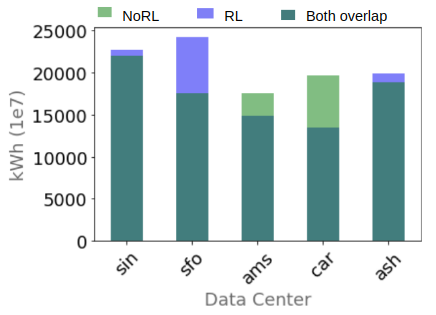
\includegraphics[scale=.50]{marginal_energy_cost/img/total_energy_comp2.png}
    \caption[Comparison of Economizer Settings in E+]{Comparison between increased economizer settings  vs. default IDF settings from \citep{kumar20} }
    \label{fig:total_energy_comp}
    \end{figure}

  The next subsection introduces the marginal costs of energy model, which will take the results from the BEM model described above.

%---------------------------------------------------------------------------------------
\subsection{Regional Marginal Costs of Energy}
%---------------------------------------------------------------------------------------
The second module requires a time-series profile of the electrical grid’s power source attributions, where the intervals of the power generation values match the BEM energy profile. The corresponding  site and regional grid model pairs are indicated in Table~\ref{table:tab02}. For this model the energy generation regional grid profiles are obtained from Platt, who provides profiles for 13 US regions in DOSCOE [5]. Singapore and Amsterdam data-centers grid profiles are constructed as described below.

\begin{table}[ht]
  \vspace{-10 pt}
  \caption{Data Center Site and Power Grid}
  \label{table:tab02}
  \centering
  \begin{tabular}{| c | c | c |  }
    \hline
    \bf{DC ID} & \bf{DC Location} & \bf{Regional Grid} \\
    \hline
    SFO & San Francisco, CA & California \\
    \hline
    CAR & Carrolton, Texas & ERCOT \\
    \hline
    ASH & Ashburn, VA & Midatlantic \\
    \hline
    AMS & Amsterdam & Netherlands \\
    \hline
    SIN & Singapore & Singapore \\
    \hline
  \end{tabular}
  \vspace{-10 pt}   % Please use appropriate negative vspace to remove the space above/below the Table
  \end{table}

  Each U.S region's grid profile is composed of hourly demands and corresponding production capacity of several power generation technologies. Hourly values for each region’s demand, solar, wind, coal, coal with cryogenic capture, coal amine gas scrubbing, and nuclear are defined. These grid regions are representative of three out of five of the data-center locations being simulated. 
  
  For Singapore, the International Energy Agency (IEA) provides a top down view of the annual energy production from various technologies. The IEA data shows that the renewable penetration in the energy supply for Singapore accounted for only 1.6\% of the total energy demand in 2016, the last year the data is available \citep{IEA17}. Due to this negligible contribution from renewable sources and lack of hourly generation data, it is assumed that all demand is met by natural gas power generators, consistent with other sources \citep{eia20}. The demand profile for Singapore in 2016 is obtained from \citep{sin16}.

  For the Amsterdam data center, energy profile of Netherlands is used. The IEA indicates that in 2018, 12\% of Netherlands's energy demands was met by renewable sources. This is a meaningful contribution from renewable, therefore a more granular generation profile is prudent as opposed to Singapore which did not require evaluations of the energy mix at any given time.  To formulate a more granular resolution of the Netherlands' generation, the IEA data is supplemented with data from the Open-Power-System-Data to characterize the time series profile of renewable energy \citep{ospd19}. OPSD provides hourly data for the renewable sources only. The balance of the energy demands in the Netherlands is met by fossil fuel-based generators, namely 35\% by coal and 42\% by natural gas \citep{eia20b}. The DOSCOE grid profiles don’t have any corresponding field for bio-mass, so the bio-mass generation indicated in OPSD is lumped in with the fossil fuel generators. In the discussion section, some validation for this approach is presented. The Netherlands also produces nuclear energy, but only the annual production rates were obtained \citep{eia20b}. In this works implementation of the DOSCOE, the annual nuclear production for Netherlands is distributed equally over the year and modeled as a constant (non-dispatchable) base load throughout the year.  

  The MEC coupled BEM algorithm is given below. In the algorithm two inputs are required. The first is DOSCOE[region], it is a two-dimensional array formatted as described in \citep{platt17}. It indicates hourly grid profiles of the power demand and power capacity of the available energy sources at the corresponding hour. The second input, traffic.language, is a one-dimensional vector indicating the network traffic to the respective site from \cite{kumar20b}. In the algorithm; for each language, it’s traffic to the respective data center is checked. If there are traces of a language routed to a site, the algorithm performs the BEM simulation by invoking EnergyPlus. This resulting demands from EnergyPlus are then added to the region’s grid demand profile. If a language does not have any traffic to a particular site than, the data center site does not do any work and the BEM simulation is bypassed.  

  \begin{algorithm}
    \begin{small}
    \caption{MEC coupled BEM algorithm}
    \begin{algorithmic}
      \REQUIRE DOSCOE[region] \& traffic.language[site]
      \FOR{site and region in DC.site and DC.region}
        \IF{traffic.language[site].all $!= 0$: }
        \STATE $DEMAND_{DC}$ \gets BEM(site, traffic.language)$
        \STATE $DOSCOE[region].demand \pluseq demand[site]$
        \ENDIF
      \ENDFOR
      \STATE $CO_{2}$ {footprint}$\ =\ GridSim(region, rps)$
      \STATE 
      \begin{small}
      \STATE{Where $DEMAND_{DC}$ is the marginal demand the data center puts on the power grid,}
      \end{small}
    \end{algorithmic}
    \label{Service Profile}
  \end{small}
  \end{algorithm}

  The second step of algorithm quantifies the marginal carbon footprint of the grid with the added data center loads by running DOSCOE’s Grid Simulator. In this step, the renewable portfolio standard (rps) argument specifies the percentage of renewable energy mix for the region.  

  In the next section the results from the methodology are discussed. 


%---------------------------------------------------------------------------------------
\section{Results \& Discussions}
%---------------------------------------------------------------------------------------
The resulting values of the carbon footprint for each data center's energy source is summarized in Table~\ref{dc_carbon_footprint}. The energy model for the 491 kW data center has been scaled by 1000 to represent the metro scale of data centers. The table further indicates the carbon footprint of each of the languages being served from the data centers. The values are indicative of the marginal $CO_{2}$ emitted by adding the data center demand to the grid.


% \begin{table*}[ht]
%   \vspace{-10 pt}
%   \caption{Data Center Carbon Footprint (Tons of CO_2)}
%   \label{table:tab03}
%   \begin{small}
%   \centering
%   \begin{tabular}{|c c c c c c c c c| }
%     \hline
%     \bf{DC ID} & \bf{de} & \bf{en}    & \bf{es} & \bf{fr} & \bf{ja} & \bf{ru} & \bf{zh} & \bf{total}\\
%     \hline
%     SFO       & 0       & 1,301,549  & 0           & 0      & 0 & 0 & 0 & \bf{1,301,549}\\
%     CAR       & 0       & 519,466    & 1,341,227  & 0       & 0 & 0 & 0 & \bf{1,860,693}\\
%     ASH       & 0       & 563,085    & 1,109,162  & 661,919 & 0 & 0 & 0 & \bf{2,334,166}\\
%     AMS       & 464,780 & 470,714    & 473,987    & 766,542 & 0 & 1,027,424 & 457,393 & \bf{3,660,840}\\
%     SIN       & 464,780 & 470,714    & 473,987    & 766,542 & 0 & 1,027,424 & 457,393 & \bf{3,660,840}\\
%     \hline
%     \bf{Sum} & \bf{464,780} & \bf{3,446,114}    & \bf{2,924,376} & \bf{2,042,611} & \bf{873,602} & \bf{1,888,019} & \bf{1,035,892} & \bf{12,675,394}\\
%     \hline
%   \end{tabular}
%   \end{small}
%   \vspace{-10 pt}   % Use appropriate negative vspace to remove the space above/below the Table
%   \end{table*}

 % \sisetup{
%   round-mode          = places, % Rounds numbers
%   round-precision     = 2, % to 2 places
% } Need to specify column type={S} to control sig figs


\begin{table*}[h!]
  \begin{center}
    \scalebox{0.8}{%
    \pgfplotstabletypeset[
      multicolumn names, % allows to have multicolumn names
      col sep=comma, % the seperator in our .csv file
      display columns/0/.style={
		column name=\textbf{Site}, % name of first columm
		string type},  % use siunitx for formatting
      display columns/1/.style={
		column name=\textbf{German},
		string type},
	  display columns/2/.style={
		column name=\textbf{English},
		string type},
	  display columns/3/.style={
		column name=\textbf{Spanish},
		string type},
	  display columns/4/.style={
		column name=\textbf{French},
		string type},
      display columns/5/.style={
		column name=\textbf{Japanese},
		string type},
	  display columns/6/.style={
		column name=\textbf{Russian},
		string type},
	  display columns/7/.style={
		column name=\textbf{Chinese},
		string type},
	  display columns/8/.style={
		column name=\textbf{Total},
		string type},
      every head row/.style={
		before row={\toprule}, % have a rule at top
		after row={
% 			\si{\ampere} & \si{\volt}\\ % the units seperated by &
			\midrule} % rule under units
			},
		every last row/.style={before row={\toprule}, after row=\bottomrule}, % rule at bottom
    ]{embodied_cost_model/contents/data/ops_co2_table3.csv} % filename/path to file
  }
  \end{center}
     \caption[Data Center Operation Carbon Footprint]{Data Center Operation Carbon Footprint (Tonnes of CO2 Emitted over the Year)}
    \label{dc_carbon_footprint}
\end{table*}



Table~ \ref{dc_carbon_footprint} indicates the total marginal carbon footprint for each language in the last row by summing the language column. While the total marginal carbon footprint of each data center is obtained by summing the rows as shown in the last column. The English pages have the most traffic globally and as expected English has the largest marginal carbon footprint due to its data-center operations. It is surprising however that the Netherlands data center has the highest total marginal carbon footprint among the data centers. A relatively lower marginal cost is expected for Netherlands due to the comparatively cooler ambient temperatures there which enables the data center systems to use economizers for more hour. The EnergyPlus results support the expected lower building energy demands for the Netherlands site as shown in the stacked PUE histogram in Figure~\ref{fig:pue}. However, the network model simulation has many languages routed to the Amsterdam data center making its absolute workload relatively higher than other data centers. The additional workloads appear to be offsetting the saving from the building operations.

\begin{figure}
  \centering
  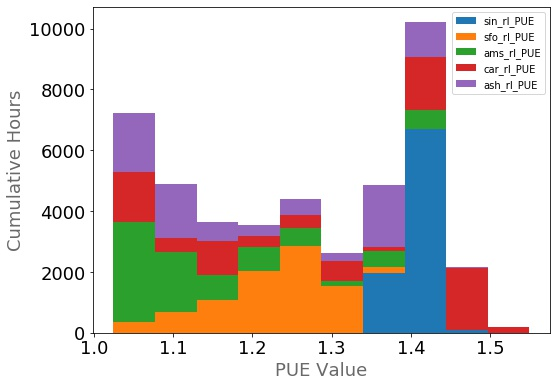
\includegraphics[scale=.40]{marginal_energy_cost/img/pue.jpg}
  \caption{Stacked histogram of PUE from all Data Centers.}
  \label{fig:pue}
  \end{figure}

Figure~\ref{fig:pue} is a histogram plot of the PUEs for all the data centers in the evaluated network. Each color in the figure represents the a specific data center. The x-axis indicates the PUE value and the y-axis indicates the the number of hours the data centers have at specific values. As a concrete example, the bars representing Netherlands site is labeled as ams-rl\_PUE and has most most hours at or below a PUE of 1.1. Other data centers also have a PUE of 1.1. Stacking the curves from the different data centers indicates the global network's time spent at a specific PUE.

The efficiency of the Netherlands site is on the lower PUE value end; the marginal carbon footprint indicated in Table~\ref{dc_carbon_footprint} can be attributed to the energy supply mix and higher network traffic from multiple languages. The constructed DOSCOE grid profile for Netherlands as described above is biased towards fossil fuels, therefore its carbon emissions are higher. This work used several secondary sources to construct the grid profile for the Netherlands and these sources may need to be validated more rigorously for future work.

As an implementation detail, the DOSCOE model proved to be quite sensitive to the data structure of the load profiles. For example any null value in the profile resulted in breaking the linear solver. Also, Solar and wind energy are required to be non-zero for at least one hour of the year. This requirement is a practical constraint, but in the profile developed for this work the values are arbitrarily set to a low value across all hours. Specifically, the defaults setting used in the work is 0.1 MW for each hour. 


%---------------------------------------------------------------------------------------
\section{Conclusion}
%---------------------------------------------------------------------------------------
The network dependencies between physically dispersed data center resources make system level building design decisions a challenge to reason about. This research has presented a quantitative method to couple the network dependencies of data centers with their building energy and grid level marginal costs of energy. As shown for the Netherlands site, lower building level efficiencies, such has PUE does not equate to lower carbon footprint.  

As pointed out in the background section, there is a lack of bottoms up building design and carbon footprint models. The modular methodology of this research is a novel means of coupling abstracted service level metrics (WAN traffic in this case) with physical based building energy simulation (EnergyPlus in this case). This integrated tool set can be used by data center system modelers to optimize their deployment across geographical bounds. Future work should consider controlling the network traffic based on building energy simulations to achieve global optimality in real time operational environments.  


